\iffalse
This file is protected by Copyright. Please refer to the COPYRIGHT file
distributed with this source distribution.

This file is part of OpenCPI <http://www.opencpi.org>

OpenCPI is free software: you can redistribute it and/or modify it under the
terms of the GNU Lesser General Public License as published by the Free Software
Foundation, either version 3 of the License, or (at your option) any later
version.

OpenCPI is distributed in the hope that it will be useful, but WITHOUT ANY
WARRANTY; without even the implied warranty of MERCHANTABILITY or FITNESS FOR A
PARTICULAR PURPOSE. See the GNU Lesser General Public License for more details.

You should have received a copy of the GNU Lesser General Public License along
with this program. If not, see <http://www.gnu.org/licenses/>.
\fi
%----------------------------------------------------------------------------------------
% Update the docTitle and docVersion per document
%----------------------------------------------------------------------------------------
\def\docTitle{Getting Started Guide}
\def\docVersion{1.5}
%----------------------------------------------------------------------------------------
\def\snippetpath{snippets}
% Usage:
% \def\snippetpath{../../../../../doc/av/tex/snippets/}
% % Usage:
% \def\snippetpath{../../../../../doc/av/tex/snippets/}
% % Usage:
% \def\snippetpath{../../../../../doc/av/tex/snippets/}
% \input{\snippetpath/includes}
% From then on, you can use "input" With no paths to get to "snippets"
% You also get all "major" snippets not part of the global LaTeX_Header
% NOTE: If not using the global LaTeX_Header, you need to
% \usepackage{ifthen} to use the \githubio macro

\hyphenation{ANGRY-VIPER} % Tell it where to hyphenate
\hyphenation{Cent-OS} % Tell it where to hyphenate
\hyphenation{install-ation} % Tell it where to hyphenate

\newcommand{\todo}[1]{\textcolor{red}{TODO: #1}\PackageWarning{TODO:}{#1}} % To do notes
\newcommand{\code}[1]{\texttt{#1}} % For inline code snippet or command line
\newcommand{\sref}[1]{Section~\ref{#1}} % To quickly reference a section

% To quickly reference a versioned PDF on github.io
% \def\ocpiversion{1.5.0}
\def\ocpiversion{1.5.0rc4} % TEMPORARY

% This gives a link to github.io document. By default, it puts the filename.
% You can optionally change the link, e.g.
% \githubio{FPGA\_Vendor\_Tools\_Installation\_Guide.pdf} vs.
% \githubio[\textit{FPGA Vendor Tools Installation Guide}]{FPGA\_Vendor\_Tools\_Installation\_Guide.pdf}
% or if you want the raw ugly URL to come out, \githubioURL{FPGA_Vendor_Tools_Installation_Guide.pdf}
\newcommand{\githubio}[2][]{% The default is for FIRST param!
\href{http://opencpi.github.io/releases/\ocpiversion/#2}{\ifthenelse{\equal{#1}{}}{\texttt{#2}}{#1}}}
\newcommand{\githubioURL}[1]{\url{http://opencpi.github.io/releases/\ocpiversion/#1}}

% Fix import paths
\makeatletter
\def\input@path{{\snippetpath/}}
\makeatother

% From then on, you can use "input" With no paths to get to "snippets"
% You also get all "major" snippets not part of the global LaTeX_Header
% NOTE: If not using the global LaTeX_Header, you need to
% \usepackage{ifthen} to use the \githubio macro

\hyphenation{ANGRY-VIPER} % Tell it where to hyphenate
\hyphenation{Cent-OS} % Tell it where to hyphenate
\hyphenation{install-ation} % Tell it where to hyphenate

\newcommand{\todo}[1]{\textcolor{red}{TODO: #1}\PackageWarning{TODO:}{#1}} % To do notes
\newcommand{\code}[1]{\texttt{#1}} % For inline code snippet or command line
\newcommand{\sref}[1]{Section~\ref{#1}} % To quickly reference a section

% To quickly reference a versioned PDF on github.io
% \def\ocpiversion{1.5.0}
\def\ocpiversion{1.5.0rc4} % TEMPORARY

% This gives a link to github.io document. By default, it puts the filename.
% You can optionally change the link, e.g.
% \githubio{FPGA\_Vendor\_Tools\_Installation\_Guide.pdf} vs.
% \githubio[\textit{FPGA Vendor Tools Installation Guide}]{FPGA\_Vendor\_Tools\_Installation\_Guide.pdf}
% or if you want the raw ugly URL to come out, \githubioURL{FPGA_Vendor_Tools_Installation_Guide.pdf}
\newcommand{\githubio}[2][]{% The default is for FIRST param!
\href{http://opencpi.github.io/releases/\ocpiversion/#2}{\ifthenelse{\equal{#1}{}}{\texttt{#2}}{#1}}}
\newcommand{\githubioURL}[1]{\url{http://opencpi.github.io/releases/\ocpiversion/#1}}

% Fix import paths
\makeatletter
\def\input@path{{\snippetpath/}}
\makeatother

% From then on, you can use "input" With no paths to get to "snippets"
% You also get all "major" snippets not part of the global LaTeX_Header
% NOTE: If not using the global LaTeX_Header, you need to
% \usepackage{ifthen} to use the \githubio macro

\hyphenation{ANGRY-VIPER} % Tell it where to hyphenate
\hyphenation{Cent-OS} % Tell it where to hyphenate
\hyphenation{install-ation} % Tell it where to hyphenate

\newcommand{\todo}[1]{\textcolor{red}{TODO: #1}\PackageWarning{TODO:}{#1}} % To do notes
\newcommand{\code}[1]{\texttt{#1}} % For inline code snippet or command line
\newcommand{\sref}[1]{Section~\ref{#1}} % To quickly reference a section

% To quickly reference a versioned PDF on github.io
% \def\ocpiversion{1.5.0}
\def\ocpiversion{1.5.0rc4} % TEMPORARY

% This gives a link to github.io document. By default, it puts the filename.
% You can optionally change the link, e.g.
% \githubio{FPGA\_Vendor\_Tools\_Installation\_Guide.pdf} vs.
% \githubio[\textit{FPGA Vendor Tools Installation Guide}]{FPGA\_Vendor\_Tools\_Installation\_Guide.pdf}
% or if you want the raw ugly URL to come out, \githubioURL{FPGA_Vendor_Tools_Installation_Guide.pdf}
\newcommand{\githubio}[2][]{% The default is for FIRST param!
\href{http://opencpi.github.io/releases/\ocpiversion/#2}{\ifthenelse{\equal{#1}{}}{\texttt{#2}}{#1}}}
\newcommand{\githubioURL}[1]{\url{http://opencpi.github.io/releases/\ocpiversion/#1}}

% Fix import paths
\makeatletter
\def\input@path{{\snippetpath/}}
\makeatother

\documentclass{article}
\iffalse
This file is protected by Copyright. Please refer to the COPYRIGHT file
distributed with this source distribution.

This file is part of OpenCPI <http://www.opencpi.org>

OpenCPI is free software: you can redistribute it and/or modify it under the
terms of the GNU Lesser General Public License as published by the Free Software
Foundation, either version 3 of the License, or (at your option) any later
version.

OpenCPI is distributed in the hope that it will be useful, but WITHOUT ANY
WARRANTY; without even the implied warranty of MERCHANTABILITY or FITNESS FOR A
PARTICULAR PURPOSE. See the GNU Lesser General Public License for more details.

You should have received a copy of the GNU Lesser General Public License along
with this program. If not, see <http://www.gnu.org/licenses/>.
\fi
\author{} % Force author to be blank
%----------------------------------------------------------------------------------------
% Paper size, orientation and margins
%----------------------------------------------------------------------------------------
\usepackage{geometry}
\geometry{
        letterpaper, % paper type
        portrait,    % text direction
        left=.75in,  % left margin
        top=.75in,   % top margin
        right=.75in, % right margin
        bottom=.75in % bottom margin
 }
%----------------------------------------------------------------------------------------
% Header/Footer
%----------------------------------------------------------------------------------------
\usepackage{fancyhdr} \pagestyle{fancy} % required for fancy headers
\renewcommand{\headrulewidth}{0.5pt}
\renewcommand{\footrulewidth}{0.5pt}
\rhead{\small{ANGRYVIPER Team}}
% \rfoot{\thepage}
%----------------------------------------------------------------------------------------
% Appendix packages
%----------------------------------------------------------------------------------------
\usepackage[toc,page]{appendix}
%----------------------------------------------------------------------------------------
% Defined Commands & Renamed Commands
%----------------------------------------------------------------------------------------
\renewcommand{\contentsname}{Table of Contents}
\renewcommand{\listfigurename}{List of Figures}
\renewcommand{\listtablename}{List of Tables}
%----------------------------------------------------------------------------------------
% Various packages
%----------------------------------------------------------------------------------------
\usepackage[usenames,dvipsnames]{xcolor} % for color names see https://en.wikibooks.org/wiki/LaTeX/Colors
\usepackage{hyperref}  % for linking urls and lists
\usepackage{graphicx}  % for including pictures by file
\usepackage{listings}  % for coding language styles
\usepackage{rotating}  % for sideways table
\usepackage{pifont}    % for sideways table
\usepackage{pdflscape} % for landscape view
\usepackage{subfig}
\usepackage{xstring}
\uchyph=0 % Never hyphenate acronyms like RCC (I think this overrides ANGRYVIPER above)
\renewcommand\_{\textunderscore\allowbreak} % Allow words to break/newline on underscores
%----------------------------------------------------------------------------------------
% Table packages
%----------------------------------------------------------------------------------------
\usepackage{longtable} % for long possibly multi-page tables
\usepackage{tabularx} % c=center,l=left,r=right,X=fill
% These define tabularx columns "C" and "R" to match "X" but center/right aligned
\newcolumntype{C}{>{\centering\arraybackslash}X}
\newcolumntype{R}{>{\raggedleft\arraybackslash}X}
\usepackage{float}
\floatstyle{plaintop}
\usepackage[tableposition=top]{caption}
\newcolumntype{P}[1]{>{\centering\arraybackslash}p{#1}}
\newcolumntype{M}[1]{>{\centering\arraybackslash}m{#1}}
%----------------------------------------------------------------------------------------
% Block Diagram / FSM Drawings
%----------------------------------------------------------------------------------------
\usepackage{tikz}
\usetikzlibrary{shapes,arrows,fit,positioning}
\usetikzlibrary{automata} % used for the fsm
%----------------------------------------------------------------------------------------
% Colors Used
%----------------------------------------------------------------------------------------
\usepackage{colortbl}
\definecolor{blue}{rgb}{.7,.8,.9}
\definecolor{ceruleanblue}{rgb}{0.16, 0.32, 0.75}
\definecolor{drkgreen}{rgb}{0,0.6,0}
\definecolor{deepmagenta}{rgb}{0.8, 0.0, 0.8}
\definecolor{cyan}{rgb}{0.0,0.6,0.6}
\definecolor{maroon}{rgb}{0.5,0,0}
%----------------------------------------------------------------------------------------
% VHDL Coding Language Style
% modified from: http://latex-community.org/forum/viewtopic.php?f=44&t=22076
%----------------------------------------------------------------------------------------
\lstdefinelanguage{VHDL}
{
        basicstyle=\ttfamily\footnotesize,
        columns=fullflexible,keepspaces,      % https://tex.stackexchange.com/a/46695/87531
        keywordstyle=\color{ceruleanblue},
        commentstyle=\color{drkgreen},
        morekeywords={
    library,use,all,entity,is,port,in,out,end,architecture,of,
    begin,and, signal, when, if, else, process, end,
        },
        morecomment=[l]--
}
%----------------------------------------------------------------------------------------
% XML Coding Language Style
% modified from: http://tex.stackexchange.com/questions/10255/xml-syntax-highlighting
%----------------------------------------------------------------------------------------
\lstdefinelanguage{XML}
{
        basicstyle=\ttfamily\footnotesize,
        columns=fullflexible,keepspaces,
        morestring=[s]{"}{"},
        morecomment=[s]{!--}{--},
        commentstyle=\color{drkgreen},
        moredelim=[s][\color{black}]{>}{<},
        moredelim=[s][\color{cyan}]{\ }{=},
        stringstyle=\color{maroon},
        identifierstyle=\color{ceruleanblue}
}
%----------------------------------------------------------------------------------------
% DIFF Coding Language Style
% modified from http://tex.stackexchange.com/questions/50176/highlighting-a-diff-file
%----------------------------------------------------------------------------------------
\lstdefinelanguage{diff}
{
        basicstyle=\ttfamily\footnotesize,
        columns=fullflexible,keepspaces,
        breaklines=true,                                % wrap text
        morecomment=[f][\color{ceruleanblue}]{@@},      % group identifier
        morecomment=[f][\color{red}]-,                  % deleted lines
        morecomment=[f][\color{drkgreen}]+,             % added lines
        morecomment=[f][\color{deepmagenta}]{---},      % Diff header lines (must appear after +,-)
        morecomment=[f][\color{deepmagenta}]{+++},
}
%----------------------------------------------------------------------------------------
% Python Coding Language Style
% modified from
%----------------------------------------------------------------------------------------
\lstdefinelanguage{python}
{
        basicstyle=\ttfamily\footnotesize,
        columns=fullflexible,keepspaces,
        keywordstyle=\color{ceruleanblue},
        commentstyle=\color{drkgreen},
        stringstyle=\color{orange},
        morekeywords={
    print, if, sys, len, from, import, as, open,close, def, main, for, else, write, read, range,
        },
        comment=[l]{\#}
}
%----------------------------------------------------------------------------------------
% Fontsize Notes in order from smallest to largest
%----------------------------------------------------------------------------------------
%    \tiny
%    \scriptsize
%    \footnotesize
%    \small
%    \normalsize
%    \large
%    \Large
%    \LARGE
%    \huge
%    \Huge

\iffalse
This file is protected by Copyright. Please refer to the COPYRIGHT file
distributed with this source distribution.

This file is part of OpenCPI <http://www.opencpi.org>

OpenCPI is free software: you can redistribute it and/or modify it under the
terms of the GNU Lesser General Public License as published by the Free Software
Foundation, either version 3 of the License, or (at your option) any later
version.

OpenCPI is distributed in the hope that it will be useful, but WITHOUT ANY
WARRANTY; without even the implied warranty of MERCHANTABILITY or FITNESS FOR A
PARTICULAR PURPOSE. See the GNU Lesser General Public License for more details.

You should have received a copy of the GNU Lesser General Public License along
with this program. If not, see <http://www.gnu.org/licenses/>.
\fi

\iffalse

This snippet defines macros to be used when describing ocpidev commands
to give the user the equivalent in the IDE. See AV-4628.

To see all output:
\code{\$ ocpidev build something something}
\OcpidevBuild
\code{\$ ocpidev clean something something}
\OcpidevClean
\code{\$ ocpidev run test something something}
\OcpidevRunTest
\code{\$ ocpidev create (no options)}
\OcpidevCreate{}
\code{\$ ocpidev create project}
\OcpidevCreate{Project}
\code{\$ ocpidev clean project Project}
\OcpidevCleanProject{Project}
\code{\$ ocpidev register project my\_proj}
\OcpidevRegisterProject{my_proj}
\code{\$ ocpidev unregister project my\_proj}
\OcpidevUnRegisterProject{my_proj}

\fi
% https://tex.stackexchange.com/a/5227
\usetikzlibrary{shadows}
\newcommand*\OcpidevKeystroke[1]{%
  \tikz[baseline=(key.base)]
    \node[%
      draw,
      fill=white,
      drop shadow={shadow xshift=0.25ex,shadow yshift=-0.25ex,fill=black,opacity=0.75},
      rectangle,
      rounded corners=2pt,
      inner sep=1pt,
      line width=0.5pt,
      font=\scriptsize\sffamily
    ](key) {#1\strut}
  ;
}

\providecommand{\OcpidevCtrlClick}{(use \OcpidevKeystroke{~Ctrl~} for multiple selection)}

\providecommand{\OcpidevTemplate}[1]{
\begin{center}
\framebox{\parbox{0.8\linewidth}{\textit{To perform this operation within the IDE:}
#1}}
\end{center}
}

% OcpidevBuild = "ocpidev build"
\providecommand{\OcpidevBuild}{\OcpidevTemplate{
\begin{enumerate}
\setlength\itemsep{0em} %tighten
\item Open the ANGRYVIPER Perspective
\item Select the asset from OpenCPI Project View
\item Import to ANGRYVIPER Operations Panel using ``$>$'' button
\item Select the RCC and/or HDL platforms for the build \OcpidevCtrlClick
\item Click ``Build''
\end{enumerate}
% Open the ANGRYVIPER Perspective, select the RCC and/or HDL platforms for the build \OcpidevCtrlClick , then select the asset in OpenCPI Projects view, right click, select build.
}}

% OcpidevClean = "ocpidev clean"
\providecommand{\OcpidevClean}{\OcpidevTemplate{
In the OpenCPI Projects view, select the project, right-click, select clean from the menu.
}}

% OcpidevRunTest = "ocpidev run test"
\providecommand{\OcpidevRunTest}{\OcpidevTemplate{
\begin{enumerate}
\setlength\itemsep{0em} %tighten
\item Click the ``Tests'' radio button and select RCC and/or HDL platforms for the run \OcpidevCtrlClick .
\item Click the ``+remotes'' button, enter the remote string, click OK.
\item Select the remote in the remotes list.
\item In the OpenCPI Projects view, select the desired unit tests, click the ``$>$'' button in the operations panel, then click the desired operation to build and then run the listed tests on the selected remote.
\end{enumerate}
}}

% OcpidevCreate = "ocpidev create <$1>"
\providecommand{\OcpidevCreate}[1]{\OcpidevTemplate{
\begin{itemize}
\setlength\itemsep{0em} %tighten
\item Place the cursor in the OpenCPI Projects panel, right click, select asset wizard.
\item Select the asset type\ifthenelse{\equal{#1}{}}{}{ (``#1'')} in the drop-down, fill in the required inputs, click finish.
\item When the process finishes, the new asset is displayed in both project views. (If the asset has an XML editor, then the editor opens.)
\end{itemize}
}}

% OcpidevCleanProject = "ocpidev clean project <$1>"
\providecommand{\OcpidevCleanProject}[1]{\OcpidevTemplate{\textit{(The project ``#1'' must be imported into the IDE and then refresh the OpenCPI Projects view so the project is shown.)}
\begin{itemize}
\setlength\itemsep{0em} %tighten
\item Right click on #1 $\Rightarrow$ ``Clean''
\end{itemize}
}}

% OcpidevRegisterProject = "ocpidev register project <$1>"
% OcpidevUnRegisterProject = "ocpidev unregister project <$1>"
\providecommand{\OcpidevRegisterProjectKernel}[2]{\OcpidevTemplate{\textit{(The project ``#1'' must be imported into the IDE and then refresh the OpenCPI Projects view so the project is shown.)}
\begin{itemize}
\setlength\itemsep{0em} %tighten
\item In the OpenCPI Projects view, select the project, right-click, select ``#2'' from the menu. (Depending on state of the project, this option may not be available.)
\end{itemize}
}}
\providecommand{\OcpidevRegisterProject}[2]{\OcpidevRegisterProjectKernel{\path{#1}}{register}}
\providecommand{\OcpidevUnRegisterProject}[2]{\OcpidevRegisterProjectKernel{\path{#1}}{unregister}}

\pagenumbering{roman}
\setlength{\parindent}{0pt} % Don't indent all paragraphs
\newcommand{\forceindent}{\leavevmode{\parindent=1em\indent}}
\date{Version \docVersion} % Force date to be blank and override date with version
\title{\docTitle}
\lhead{\small {\docTitle} }
%----------------------------------------------------------------------------------------
% This makes sure that our verbatim blocks don't get pagebreaks in them
\def\bstart{~\\
\begin{minipage}{\linewidth}}
\def\bend{\end{minipage}
~\\
}
\usepackage{listings}
\usepackage{xcolor}
\usepackage{textcomp}
\begin{document}
\maketitle
% \thispagestyle{fancy}
\newpage

        \begin{center}
        \textit{\textbf{Revision History}}
                \begin{table}[H]
                \label{table:revisions} % Add "[H]" to force placement of table
                        \begin{tabularx}{\textwidth}{|c|X|l|}
                        \hline
                        \rowcolor{blue}
                        \textbf{Revision} & \textbf{Description of Change} & \textbf{Date} \\
                        \hline
                        v1.0 & Initial creation & 2/2016 \\
                        \hline
                        v1.1 & Updated for OpenCPI Release 1.1 & 3/2017 \\
                        \hline
                        v1.2 & Updated for OpenCPI Release 1.2 & 8/2017 \\
                        \hline
                        v1.3 & Updated for OpenCPI Release 1.3 & 2/2018 \\
                        \hline
                        v1.4 & Updated for OpenCPI Release 1.4 & 10/2018 \\
                        \hline
                        v1.5 & Updated for OpenCPI Release 1.5 & 4/2019 \\
                        \hline
                        \end{tabularx}
                \end{table}
        \end{center}

\newpage
\tableofcontents
\newpage
\listoffigures
\newpage
\listoftables
\newpage
\pagenumbering{arabic}
\section{References}

This document assumes a basic understanding of the Linux command line environment. It does not require a working knowledge of OpenCPI.
\def\refskipgs{} % Skip self
\def\myreferences{
\hline
Component Development Guide &
\githubio{OpenCPI\_Component\_Development.pdf} \\
\hline
RCC Development Guide &
\githubio{OpenCPI\_RCC\_Development.pdf} \\
\hline
HDL Development Guide &
\githubio{OpenCPI\_HDL\_Development.pdf} \\
}
\iffalse
This file is protected by Copyright. Please refer to the COPYRIGHT file
distributed with this source distribution.

This file is part of OpenCPI <http://www.opencpi.org>

OpenCPI is free software: you can redistribute it and/or modify it under the
terms of the GNU Lesser General Public License as published by the Free Software
Foundation, either version 3 of the License, or (at your option) any later
version.

OpenCPI is distributed in the hope that it will be useful, but WITHOUT ANY
WARRANTY; without even the implied warranty of MERCHANTABILITY or FITNESS FOR A
PARTICULAR PURPOSE. See the GNU Lesser General Public License for more details.

You should have received a copy of the GNU Lesser General Public License along
with this program. If not, see <http://www.gnu.org/licenses/>.
\fi

% This snippet creates the "References" table labeled "table:references"
% It creates three columns: Name, Publisher, Link and then inserts default documents
%
% To skip these defaults, define macros named
% refskipgs to skip "Getting Started"
% refskipig to skip "Installation Guide"
% refskipac to skip "Acronyms and Definitions"
% refskipocpiov to skip "OpenCPI Overview"
%
% See RPM_Installation_Guide.tex for examples
%
% After the defaults, it optionally inserts the "myreferences" macro that
% you defined elsewhere (you put hlines above all lines)
%
% If you want the \caption on the bottom, define "refcapbottom"
\begin{center}
\renewcommand*\footnoterule{} % Remove separator line from footnote
\renewcommand{\thempfootnote}{\arabic{mpfootnote}} % Use Arabic numbers (or can't reuse)
\begin{minipage}{0.9\textwidth}
  \begin{table}[H]
\ifx\refcapbottom\undefined
  \caption {References}
  \label{table:references}
\fi
  \begin{tabularx}{\textwidth}{|C|C|}
    \hline
    \rowcolor{blue}
    \textbf{Title} & \textbf{Link} \\
\ifx\refskipocpiov\undefined
    \hline
    OpenCPI Overview & \githubio{Overview.pdf} \\
\fi
\ifx\refskipac\undefined
    \hline
    Acronyms and Definitions & \githubio{Acronyms\_and\_Definitions.pdf} \\
\fi
\ifx\refskipgs\undefined
    \hline
    Getting Started & \githubio{Getting\_Started.pdf} \\
\fi
\ifx\refskipig\undefined
    \hline
    Installation Guide & \githubio{RPM\_Installation\_Guide.pdf} \\
\fi
\ifx\myreferences\undefined
\else
    \myreferences
\fi
    \hline
  \end{tabularx}
\ifx\refcapbottom\undefined
\else
  \caption {References}
  \label{table:references}
\fi
  \end{table}
\end{minipage}
\end{center}


\newpage
\section{Overview of OpenCPI}
Open Component Portability Infrastructure (OpenCPI) is a series of tools and runtime platform for developing and deploying heterogeneous applications.
It includes:
\begin{itemize}
\item A runtime environment to manage and deploy assets in both software and HDL.
\item A set of tools for development of applications and components for software and HDL.
\item A framework and methodology for targeting mixed processor architecture types.
\item A set of HDL and software building blocks for developers to use and expand.
\item A series of reference applications running on base platforms.
\end{itemize}

Assets and applications developed using OpenCPI are meant to simplify complex integration and improve code portability of heterogeneous solutions.
OpenCPI extends component-based architectures into GPPs and FPGAs to decrease development costs and time to market through code portability, reuse, and ease of integration.\\

For more information, consult the \textit{Overview} found in Table~\ref{table:references}.

\subsection{Projects Overview}
Historically, all OpenCPI development, for both the core team and the end user, has been within a single directory structure. As the team size and user base expand, this quickly becomes untenable, especially when taking version control systems into account. The previous working area has been broken into several locations. \\

The CDK and the source for the Core and Assets Projects are provided by the ANGRYVIPER Team (\textit{cf}. \sref{subsec:what_is_angryviper}) in the form of various RPMs that can be installed by a System Administrator.
% A version of the Core Project is provided containing prebuilt software necessary for all OpenCPI execution (and optionally development).
In order to exercise any of the supported platforms, a user must have a writable copy of the Core project in order to build HDL using his/her own specific FPGA tool version(s).

\begin{center}
\begin{table}[h]
\caption{Project Types}
%\captionof{table}{\text{Project Types}}
\begin{tabularx}{\textwidth}{|c|C|C|}
\hline
\rowcolor{blue}
Name & Contents & Expectation/Usage\\
\hline
CDK & Framework, Utilities & End-user will use, not modified
\\
\hline
Core Project & Minimal Components, Primitives, RCC Platforms, HDL Simulator Platforms & End-user will build, not modify
\\
\hline
Assets Project & Applications, Components, Primitives, Platforms, Cards/Slots, Devices, Assemblies  & End-user will build, run, maybe modify
\\
\hline
BSP Project & Platforms, Cards/Slots, Devices, etc.  & End-user will build, not modify
\\
\hline
User Project & User-provided Components, Applications, etc. & End-user will build, run, modify
\\
\hline
\end{tabularx}
\end{table}
\end{center}

\subsection{What is the ANGRYVIPER Team?}
\label{subsec:what_is_angryviper}
The ANGRYVIPER Team is a group of engineers contracted to support the OpenCPI framework with additional features, reference assets (known as \textbf{\texttt{ocpi.assets}}), additional API, RPM-based modular installation, and an integrated development environment (IDE).

\newpage
\section{A Brief overview OpenCPI's Architecture}
In this section, the basics of the framework are discussed including the communications, control, and data exchange.
\label{sec:brief_ow_arch}
At the highest level, the architecture of the framework is connectivity between three key concepts:
\begin{itemize}
\item \textbf{Application Management Model}: How component-based applications are managed and controlled including loading, launching, starting, stopping, configuring, querying, etc. This is sometimes described as how component-based applications are deployed.
\item \textbf{Authoring Model:} How components are written in order to be effective on various
processing technologies and execution environments.
\item \textbf{Data Transport:} How messages are moved between one component and another.
\end{itemize}

The core software is structured to allow extensions in any of these three dimensions: enable new management models, add new authoring models, and adding new data transport technologies. \newline

Figure~\ref{fig:what_is_opencpi} represents the conceptual plug and play functionality OpenCPI brings through the use of extensions.
These extensions can take the form of management models, new authoring models and new data technologies.

\begin{figure}[h]
\centerline{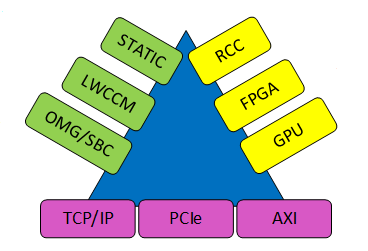
\includegraphics[scale=0.75]{./figures/pillars_of_ocpi.png}}
\caption{Conceptual extensibility of the OpenCPI framework for new and expanding target bases. Reflecting the three key concepts: Application Management, Authoring Model, and Data Transport.}
\label{fig:what_is_opencpi}
\end{figure}

\subsection{Management Models}
\label{subsec:Mangement_models}
The basis for the management model is to specify how applications are managed and deployed, including how a control application would statically or dynamically decide to execute one or more component-based applications on a given system.
The framework provides two different modes:
The first is an application called \verb+ocpirun+, which takes an application XML and control commands to execute.
The second is through the use of native C++ API for controlling and launching applications which gives the application developer a greater level of control, including reading and writing properties during execution.

\subsection{Authoring Models}
\label{subsec:Authoring_Models}
The framework uses the concept of ``containers'' which can host and execute workers. These workers can be hardware-oriented (VHDL within an FPGA) or software-oriented (C/C++ on a GPP\footnote{Standalone CPU or embedded within an FPGA as an SoC}).

\subsection{Data Transport}
\label{subsec:Data_Transport}
The communication model is conceptually based on a protocol model where a component is defined to be able to send or receive messages
with defined payloads.
The protocol can be as simple as ``frames of 200 16-bit unsigned integers''.
It can also be a variety of messages in a variety of formats based on variable length data types.
The transport mechanism can be:
\begin{itemize}
\item Passing buffer pointers with no data copying between co-located workers in software.
\item Directly connecting wires from one FPGA worker to another.
\item Moving messages over network sockets (TCP/IP).
\item Moving messages between processors using standard buses (PCIe or AXI).
\end{itemize}

The benefit here is a flexible and transparent methodology for moving data of differing types from worker to worker. This enables a simplified and abstracted development process that greatly removes the hardware implementation from the application.

\newpage
\section{Getting Started}
This section will walk through building the Core and Assets Project and all the fundamental steps of creating, building, running, and testing a simple application containing HDL workers. In the \textit{OpenCPI Component Development Guide}, the \verb+ocpidev+ command line tool is discussed in detail, but this example will serve as an introduction to using the \verb+ocpidev+ command line tool.

\subsection{Installation of OpenCPI}
The most direct method for installation of the OpenCPI framework and IDE is through the use of the OpenCPI RPMs\footnote{
% AV-5582
An alternative ``source build'' is also available for advanced usage and is documented in the \githubio[\textit{OpenCPI Installation Guide}]{OpenCPI\_Installation.pdf} -- that style of installation is not supported by this document.
}.
The RPMs allows for a normalized installation process with the inclusion of all dependencies required. A detailed installation process can be found in the \textit{RPM Installation Guide}.

\begin{center}
% AV-5582 TELL THEM AGAIN BECAUSE THEY DON'T LISTEN
\framebox{\parbox{0.8\linewidth}{\centering
\textbf{ The remainder of this document assumes the RPMs have been installed.}\\
The user's environmental variables must also be configured to build with the Xilinx Vivado software.
For more information on Vivado installation/licensing and OpenCPI environment configuration, see the \textit{FPGA Vendor Tools Installation Guide}.}}
\end{center}

\subsection{Environmental Variables}
Various environmental variables are used to control OpenCPI.
When installed, the RPMs provide ``sane'' defaults for all, with \path{OCPI_PROJECT_REGISTRY_DIR} and \path{OCPI_LIBRARY_PATH} often the only ones an end user will need to modify.
However, the ones listed in Table~\ref{table:variables} are often useful for debugging purposes.

	\begin{center}
		\begin{table}[H]
		\caption {Commonly Used Variables}\label{tab:env}
		\label{table:variables}
			\begin{tabularx}{\textwidth}{|c|X|}
\hline
\rowcolor{blue}\textbf{Variable} & \multicolumn{1}{|c|}{\textbf{Description}} \\
\hline
\path{OCPI_CDK_DIR} &
The location of the CDK's installation. If unset, many scripts and programs will fail to operate. With RPM installation, it is \textit{always} \path{/opt/opencpi/cdk}.\\
\hline
\path{OCPI_LIBRARY_PATH} &
The set of locations (or projects) used to find runtime artifacts. \textit{Every file within every path} in this colon-separated list is opened and examined for deployment metadata. For this reason, it is best to point to each projects' \path{exports} subdirectory and not their root location.\\
\hline
\path{OCPI_LOG_LEVEL} &
The amount of logging output by the runtime system. The default is zero (\textbf{0}), indicating no logging output. The maximum logging is \textbf{20}. Commonly useful startup and diagnostic information (\textit{e.g.} artifact discovery feedback) is provided at log level \textbf{8}. Unusual events are logged at level \textbf{4}.\\
\hline
\path{OCPI_PROJECT_PATH} &
The set of projects used to find various artifacts and support infrastructure \textit{during build time}. This colon-separated list is legacy (but still supported) and largely replaced by the project registry (detailed below).\\
\hline
\path{OCPI_PROJECT_REGISTRY_DIR} &
Override the default location of the project registry. If this is not set, the default project registry is OCPI\_CDK\_DIR/../project-registry.\\
\hline
\path{OCPI_SYSTEM_CONFIG} &
The runtime system XML configuration file. Default is \path{/opt/opencpi/system.xml} with a fallback to \path{/opt/opencpi/cdk/default-system.xml}.\\
\hline
			\end{tabularx}
		\end{table}
	\end{center}
\subsection{Project Registry}
A project registry is a directory that contains references to projects in a development environment. By registering a project, a user is publishing his project so it can be referenced/searched by any other project using that same project registry. The default project registry is explained in the OCPI\_PROJECT\_REGISTRY\_DIR row of Table \ref{tab:env}. To add a project to the default project registry in an RPM environment, a user needs to be in the \code{opencpi} user group. This is described in detail the \textit{RPM Installation Guide}. \\

\textbf{The sharing of projects across users with a common registry has been known to be fragile for various reasons (\textit{e.g.} incorrect permission settings, default ``umask'' values, etc.) and is \textit{not} recommended for new users.} \\

\textit{Note}: This section is informational / reference; you will create your personal registry below (\sref{sec:create_projects}). \\

The \verb+ocpidev register project+ command is used to register a project.\\
\OcpidevRegisterProject{my_proj} \\
This is done automatically when the first copies of the core and assets projects are created.
For user-provided projects (or new copies/overrides of the core/assets projects), the \code{register} command can be used.
\code{unregister} can be used to remove an existing project from the registry.%
\footnote{Note that \code{unregister} does not remove your project, it just delists it from the registry}\\

\OcpidevUnRegisterProject{my_proj}

The project registry must also be set on a per-project basis using \code{ocpidev set registry <registry-location>} to ``point back'' to the registry. See \code{ocpidev --help set} for more information.

\subsection{Set Up Work Environment (Projects and Registry)}
\subsubsection{Create Registry and Projects}
\label{sec:create_projects}
With the \texttt{opencpi-devel} rpm installed, a \texttt{core} and \texttt{assets} project can be created. It is recommended that each user has his/her own copy of the \texttt{core} and \texttt{assets} projects. Included with the CDK is an installation script, \path{ocpi-copy-projects}.
This script will copy all of the read-only projects out of \path{/opt/opencpi/projects/} and into another location.
The script takes two parameters: destination location for copied projects and the registry location where copied projects are registered (defaulting to \path{/opt/opencpi/project-registry} or \path{OCPI_PROJECT_REGISTRY_DIR}). The recommended destination location is \verb+~/ocpi_projects+. \\
% Before running this script, make sure the user is a member of the \code{opencpi} group as explained in the \textit{RPM Installation Guide}.\\

If no arguments are given, the script is interactive and the user is required to
input required information. \textit{It is recommended that the user uses interactive mode.} In interactive mode, the user is able to do the
following:
\begin{enumerate}
\item Unregister any projects from the destination registry if they choose
\item Create a new registry (recommended)
\item Update \path{.bashrc} to set the environment variable \path{OCPI_PROJECT_REGISTRY_DIR} to the destination registry
\end{enumerate}

\verb+% ocpi-copy-projects+ \\

This command may produce a handful of warnings. It is likely that these warnings can be ignored. If the command actually outputs an Error, it is likely because the user is not a member of the \code{opencpi} group in an RPM environment with a shared registry.\\

After execution, you will be reminded that \path{OCPI_PROJECT_REGISTRY_DIR} \textit{must be set} to use this new registry. You can open a new terminal and ensure it is set if the script edited \path{.bashrc} for you.
If you don't want to at this time, you must at least execute the \path{export} command given \textit{before continuing or opening the IDE}.\\

\subsubsection{Display Installed Projects}
To confirm which projects are installed and where they live, the command \texttt{ocpidev show projects} can be used.
\subsubsection{Building Projects}
\label{subsubsec:buildworkers}
In this step, the Project's contents will be built. Before completing the remaining steps, the environment must be set up as described in the \textit{RPM Installation Guide}.\\

To build a project, first pick the desired \textit{Platform} to build for. The available options are listed in Table~\ref{table:hdlworkers}.\\

The relationships between vendor tools and targets (i.e. platforms) is discussed in the \githubio{FPGA\_Vendor\_Tools\_Installation\_Guide.pdf}
	\begin{center}
		\renewcommand*\footnoterule{} % Remove separator line from footnote
		\renewcommand{\thempfootnote}{\arabic{mpfootnote}} % Use Arabic numbers (or can't reuse)
		\begin{minipage}{1.063\textwidth}
		\begin{table}[H]
		\caption {Supported Platforms}\label{tab:plats}
		\label{table:hdlworkers} % Add "[H]" to force placement of table
			\begin{tabularx}{\textwidth}{|l|l|l|p{5cm}|}
			\hline
			\rowcolor{blue}
			\textbf{Simulator Vendor} & \textbf{Platform Name} & \textbf{Project Package-ID \footnote{The Project Package-ID is the unique identifier for a project. Please reference the \textit{Component Development Guide} for more details}} & \textbf{Link}\\

			\hline
			ModelSim DE 10.6a/10.4c & \code{modelsim} & \code{ocpi.core} & \url{https://www.mentor.com/products/fv/modelsim/}\\
			\hline
			Xilinx Vivado 2017.1 & \code{xsim} & \code{ocpi.core} & \url{https://www.xilinx.com/support/download/index.html/content/xilinx/en/downloadNav/vivado-design-tools.html}\\
			\hline
			Xilinx ISE 14.7 & \code{isim} & \code{ocpi.core} & \url{https://www.xilinx.com/support/download/index.html/content/xilinx/en/downloadNav/design-tools.html}\\
			\hline
			\rowcolor{blue}
			\textbf{Hardware Platform} & \textbf{Platform Name} & \textbf{Project Package-ID} & \textbf{Link}\\
			\hline
			Epiq Solutions Matchstiq-Z1 & \code{matchstiq\_z1}\footnote{Reference the Matchstiq-Z1 Getting Started Guide to build for \code{matchstiq\_z1}} & \code{ocpi.assets} & \url{https://epiqsolutions.com/matchstiq/} \\
			\hline
			Avnet ZedBoard (Vivado build) & \code{zed}\footnote{Reference the Zedboard Getting Started Guide to build for \code{zedboard}} & \code{ocpi.assets} & \url{http://zedboard.org/}\\
			\hline
			Avnet ZedBoard (ISE build) & \code{zed\_ise}\footnote{Use Xilinx ISE tools to build for this platform} & \code{ocpi.assets} & \url{http://zedboard.org/}\\
			\hline
			Altera Stratix IV GX & \code{alst4} & \code{ocpi.assets} & \url{https://www.intel.com/content/www/us/en/products/programmable/fpga/stratix-iv.html}\\
			\hline
			Xilinx ML605 (Virtex-6) & \code{ml605} & \code{ocpi.assets} & \url{https://www.xilinx.com/products/boards-and-kits/ek-v6-ml605-g.html}\\
			\hline
			Ettus USRP E310 & \code{e3xx} & \code{ocpi.bsp.e310} & \url{https://www.ettus.com/product/details/E310-KIT}\\
			\hline
			\rowcolor{blue}
			\textbf{Software Platform} & \textbf{Platform Name} & \textbf{Project Package-ID} & \textbf{Link}\\
			\hline
			Centos6 & \code{centos6} & \code{ocpi.core} & \url{https://www.centos.org/}\\
			\hline
			Centos7 & \code{centos7} & \code{ocpi.core} & \url{https://www.centos.org/}\\
			\hline
			Xilinx Linux (xilinx-v2013.4 release) & \code{xilinx13\_3}\footnote{RCC platform associated with the zedboard and matchstiq\_z1 platforms} & \code{ocpi.core} & \url{https://github.com/Xilinx/linux-xlnx/releases/tag/xilinx-v2013.4}\\
			\hline
			Xilinx Linux (xilinx-v14.7 release) & \code{xilinx13\_4}\footnote{RCC platform associated with the e310 platform} & \code{ocpi.core} & \url{https://github.com/Xilinx/linux-xlnx/releases/tag/xilinx-v14.7}\\
			\hline
			\end{tabularx}
		\end{table}
		\end{minipage}
	\end{center}

\subsubsection{Build Core Project}
This section presents a handful of commands that can be used to build for various platforms. To complete this Guide using the \code{xsim} simulator, use the build command in the box at the end of this section.
\begin{center}
\framebox{\parbox{0.8\linewidth}{\centering The steps in this section are specific to the \code{xsim} simulator, which is installed as part as the Xilinx Vivado software. For more information on Vivado installation/licensing and OpenCPI environment configuration, see the \textit{FPGA Vendor Tools Installation Guide}.}}
\end{center}

Note that all build commands in this Guide can optionally be performed using the ANGRYVIPER IDE instead of ``\code{ocpidev build}''.\\

To build the RCC workers, go to the \texttt{core} project and run:\\ \\
\# If user will later target the Zedboard or Matchstiq-Z1:\\
\code{\% ocpidev build -\--rcc -\--rcc-platform xilinx13\_3 }\\
\OcpidevBuild

\# If user will later target the Zedboard and/or Centos7:\\
\code{\% ocpidev build -\--rcc -\--rcc-platform xilinx13\_3 -\--rcc-platform centos7}\\

The \texttt{--rcc-platform} option specifies the RCC platform to the build for.\\

Use the following \verb+ocpidev+ command to build the project for the desired platform using the information from Table~\ref{table:hdlworkers}.\\

\code{\% ocpidev build --rcc-platform <platform name> --hdl-platform <platform name>} \\

Building for multiple platforms can be combined into a single \texttt{ocpidev} call, \textit{e.g.}:\\

\code{\% ocpidev build --hdl-platform modelsim --hdl-platform xsim --hdl-platform isim --rcc-platform centos7 --rcc-platform xilinx13\_3} \\

In the \texttt{core} project, the last operation this command performs is to build the project's \texttt{hdl platforms}. You can be sure it succeeded if the last few sections of output are ``\texttt{=======Building platform xsim}''.\\
\begin{center}
\framebox{\parbox{0.8\linewidth}{\centering For the example in Section~\ref{sec:basic_example}, you \textit{must} build for \texttt{xsim} at a minimum. This takes approximately 10 minutes:\newline

\code{ocpidev build --hdl-platform xsim} \newline

\footnotesize{\textit{Note: }If you have ISE installed instead of Vivado, you can follow this guide using \code{isim} instead of \code{xsim}}
}}
\end{center}


\subsubsection{Build Assets Project}
Refer to table \ref{tab:plats} to determine whether the platform being built for lives in the \code{ocpi.assets} project. If so, follow the same building procedures documented in \sref{subsubsec:buildworkers} for the same platforms. The last assets built in the \texttt{assets} project are \texttt{applications}. You can be sure it succeeded if the last few sections of output include ``\texttt{========Building apps cic\_int\_dc\_offset\_iq\_imbalance\_mixer\_cic\_dec}''.\\

If the \code{xsim} platform is being used, the \code{ocpi.assets} project does \textit{not} need to be built at this time.\\

\newpage
\section{Creating a New Example Application}
\label{sec:basic_example}
\subsection{Overview}
This simple application will contain three HDL Workers: \verb+ramp+, \verb+square+, and \verb+ander+, which can be seen in Figure~\ref{fig:simple_app_diagram}. \newline

\begin{figure}[h]
        \centering
        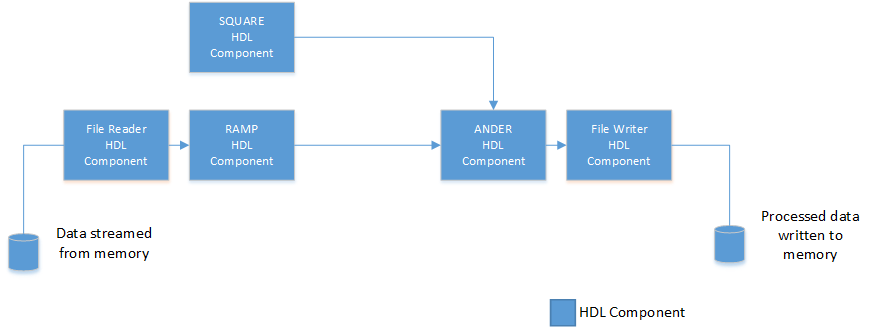
\includegraphics[scale=0.5]{./figures/simple_app_block_diagram.png}
        \caption{Block diagram of simple HDL application with three user-defined workers, a \code{FileRead}, and a \code{FileWrite}.}
        \label{fig:simple_app_diagram}
\end{figure}
For testing and simulation purposes, the OpenCPI \verb+file_read+ and \verb+file_write+ workers will be used to read input data from, and write output data to, files on the system.\newline

The basic format of an \verb+ocpidev+ command is ``\verb+ocpidev [options] <verb> <noun> <name>+''.
For this demonstration, the following \verb+nouns+ will be used: \verb+project+, \verb+library+, \verb+spec+, \verb+worker+, \verb+hdl assembly+, and \verb+application+.
\path{ocpidev} supports ``tab-completion'' for \textit{most} options, including platform names.
It is recommended that the user take advantage of this capability when performing these examples to help get a feel for the options available from the tool.
\newline

The full list of \verb+ocpidev+ verbs, nouns and options can be explored via \code{ocpidev --help}, \code{ocpidev --help <verb>}, or the \textit{OpenCPI Component Development Guide}.

\subsection{Create a Project}
Choose the name ``DemoProject'' for this project. To create the ``DemoProject'' project use the following \verb+ocpidev+ command:\\

\forceindent\verb+% ocpidev create project --register DemoProject+\\
\OcpidevCreate{Project}

The project that was just created should have also been registered.
% This assumes the default registry is being used \textit{and} the user is a member of the \code{opencpi} group (as explained in the \textit{RPM Installation Guide}.
The project registration can be done separately using the following \verb+ocpidev+ command from within the project:\\

\forceindent\forceindent\verb+% ocpidev register project+\\
\OcpidevRegisterProject{DemoProject}

Observe the directory structure created, as well as the files.\\

\bstart
\begin{verbatim}
$ tree --charset ascii DemoProject
|-- exports
|   |-- imports -> ../imports
|   `-- project-package-id
|-- imports -> /opt/opencpi/project-registry
|-- Makefile
|-- Project.exports
|-- Project.mk
`-- project.xml
3 directories, 5 files
\end{verbatim}
\bend
Change directories into ``DemoProject''.

\subsection{Create a Library}
A library is a convenient way of grouping workers. For a simple case, the framework defaults to a \verb+components+ directory as the library. To create the default ``components'' library, use the following \verb+ocpidev+ command:\\

\forceindent\verb+% ocpidev create library components+\\
\OcpidevCreate{}

\bstart
Observe the directory structure created, as well as the files:
\begin{verbatim}
DemoProject
|-- components
|   |-- lib
|   |   |-- package-id
|   |   `-- workers
|   |-- Library.mk
|   `-- Makefile
|-- exports
|   |-- imports -> ../imports
|   `-- project-package-id
|-- imports -> /opt/opencpi/project-registry
|-- Makefile
|-- Project.exports
|-- Project.mk
`-- project.xml

\end{verbatim}
\bend
For more advanced projects, one or more libraries would be placed within the \verb+components+ directory. This usage is highly recommended and explained in the \textit{OpenCPI Component Development Guide}.

\subsection{Create Components}
\textit{Components} are black boxes that dictate what properties and interfaces are implemented. A single implementation of a \textit{component} is referred to as a \textit{worker}, which is discussed in the next section. \textit{Components} are defined by an OpenCPI Component Specification (OCS). The OCS is commonly referred to as the \textit{spec file} or \textit{spec}. Each \textit{spec} includes the details that are to be \textbf{consistent among different authoring models}; meaning that if there are various implementations of a single \textit{component}, \textit{e.g.} a software (RCC) worker and an HDL worker, both \textit{workers} expect the same input and both should have the same output regardless of which architecture the worker runs on.\newline

This application requires three \textit{components}, so three \textit{specs} will be generated. To create the three template \textit{specs} use the following \verb+ocpidev+ commands:\\

\forceindent\verb+% ocpidev create component ramp+

\forceindent\verb+% ocpidev create component square+

\forceindent\verb+% ocpidev create component ander+\\
\OcpidevCreate{}

\bstart
\begin{verbatim}
DemoProject
|-- components
|   |-- lib
|   |   |-- ander-spec.xml -> ../specs/ander-spec.xml
|   |   |-- package-id
|   |   |-- ramp-spec.xml -> ../specs/ramp-spec.xml
|   |   |-- square-spec.xml -> ../specs/square-spec.xml
|   |   `-- workers
|   |-- Library.mk
|   |-- Makefile
|   `-- specs
|       |-- ander-spec.xml
|       |-- ramp-spec.xml
|       `-- square-spec.xml
|-- exports
|   |-- imports -> ../imports
|   `-- project-package-id
|-- imports -> /opt/opencpi/project-registry
|-- Makefile
|-- Project.exports
|-- Project.mk
`-- project
\end{verbatim}
\bend
Notice that three \textit{spec} templates were generated. Also note that \textit{spec files} can be easily identified by their \verb+-spec+ postfix\footnote{Some older spec files use \texttt{\_spec} as well.}. In between the \verb+ComponentSpec+ XML tags, the \textit{component} properties and interfaces need to be defined. \textbf{Every component interface (or \textit{port}) must define the direction and format of the messages they will send or receive.} This formatting is known as the \textit{protocol}, and for this example, we will use \texttt{rstream}, which is a stream of up to 4096 16-bit samples per message.

\bstart
For the \verb+ramp+ \textit{component}, insert the following XML snippet in between the \verb+ComponentSpec+ XML tags:

\begin{lstlisting}[language=xml]
<Port Name="in" Producer="false" Protocol="rstream_protocol.xml"/>
<Port Name="out" Producer="true" Protocol="rstream_protocol.xml"/>
\end{lstlisting}
\bend
\bstart
For the \verb+square+ \textit{component}, insert the following XML snippet in between the \verb+ComponentSpec+ XML tags:

\begin{lstlisting}[language=xml]
<Port Name="out" Producer="true" Protocol="rstream_protocol.xml"/>
\end{lstlisting}
\bend
\bstart
For the \verb+ander+ \textit{component}, insert the following XML snippet in between the \verb+ComponentSpec+ XML tags:

\begin{lstlisting}[language=xml]
<Port Name="in1" Producer="false" Protocol="rstream_protocol.xml"/>
<Port Name="in2" Producer="false" Protocol="rstream_protocol.xml"/>
<Port Name="out" Producer="true" Protocol="iqstream_protocol.xml"/>
\end{lstlisting}
\bend
For more details, see the \textit{OpenCPI Component Development Guide}. Now that the \textit{specs} are defined, the next step is to create the \textit{workers}.

\subsection{Create Workers}
As mentioned in the previous section, \textit{workers} are specific implementations of \textit{components}. More than one \textit{worker} can implement a \textit{component}. For this example, only one implementation per \textit{component} will be used, and each of these \textit{workers} are \textit{HDL Workers}. More details about \textit{HDL Workers} can be found in the \textit{OpenCPI HDL Development Guide}.
This example does not use any \textit{RCC (Software) Workers}, but more details about them can be found in the \textit{OpenCPI RCC Development Guide}.\newline

When creating \textit{workers}, two options need to be defined, one implicitly and one explicitly. The type of \textit{worker} is defined implicitly by appending either \verb+.rcc+ or \verb+.hdl+ to the name of the \textit{worker}. \textit{HDL Workers} use the general format for the \textit{worker} names: \verb+worker_name.hdl+. The language of the \textit{worker} can be explicitly defined; for \textit{RCC Workers} there are currently two choices: C++ or C.\newline

To create the \textit{HDL Workers}, use the following \verb+ocpidev+ commands:\\

\forceindent\verb+% ocpidev create worker ramp.hdl+

\forceindent\verb+% ocpidev create worker square.hdl+

\forceindent\verb+% ocpidev create worker ander.hdl+\\

\OcpidevCreate{}

Notice that the creation of the \verb+ramp+, \verb+square+, and \verb+ander+ \textit{HDL Workers} generated a \verb+.hdl+ directory for each. Each of the \verb+.hdl+ directories contain that \textit{worker}'s \textit{OpenCPI Worker Description} (OWD), which can be identified by the following format: \verb+worker_name.xml+. The OWD is where that \textit{worker's} specific properties and port protocols are defined. The definitions in the OWD are specific to each individual worker and may override a set of attributes defined in the OCS. Later the OWD will be edited for each \textit{worker}.\newline

Observe that in each of the \verb+.hdl+ directories there is also the \textit{skeleton file} or \textit{wrapper} in the language that was specified. In this case, the \verb+worker_name.vhd+ is the \textit{skeleton file} for the language option VHDL. Later, the \textit{skeleton file} will be edited for each \textit{worker}.\newline

The \verb+gen+ directory contains other important code that is generated from the framework and will not need to be edited. For more details see the \textit{OpenCPI Component Guide}.\\

\bstart
The project should now look similar to the following:
\begin{verbatim}
DemoProject/
|-- components
|   |-- ander.hdl
|   |   |-- ander.vhd
|   |   |-- ander.xml
|   |   |-- gen
|   |   |   |-- ander-build.xml
|   |   |   |-- ander-defs.vhd
|   |   |   |-- ander-defs.vhd.deps
|   |   |   |-- ander-impl.vhd
|   |   |   |-- ander-impl.vhd.deps
|   |   |   |-- ander.mk
|   |   |   |-- ander-skel.vhd
|   |   |   `-- ander-skel.vhd.deps
|   |   `-- Makefile
|   |-- lib
|   |   |-- ...
|   |   `-- workers
...
|   |-- ramp.hdl
|   |   |-- gen
|   |   |   |-- ramp-build.xml
|   |   |   |-- ramp-defs.vhd
|   |   |   |-- ramp-defs.vhd.deps
|   |   |   |-- ramp-impl.vhd
|   |   |   |-- ramp-impl.vhd.deps
|   |   |   |-- ramp.mk
|   |   |   |-- ramp-skel.vhd
|   |   |   `-- ramp-skel.vhd.deps
|   |   |-- Makefile
|   |   |-- ramp.vhd
|   |   `-- ramp.xml
|   |-- specs
|   |   |-- ander-spec.xml
|   |   |-- ramp-spec.xml
|   |   `-- square-spec.xml
|   `-- square.hdl
|       |-- gen
|       |   |-- square-build.xml
|       |   |-- square-defs.vhd
|       |   |-- square-defs.vhd.deps
|       |   |-- square-impl.vhd
|       |   |-- square-impl.vhd.deps
|       |   |-- square.mk
|       |   |-- square-skel.vhd
|       |   `-- square-skel.vhd.deps
|       |-- Makefile
|       |-- square.vhd
|       `-- square.xml
...
\end{verbatim}
\bend
\bstart
However, if you are using version control\footnote{The \path{lib}, \path{imports}, and \path{exports} should not be in SCM.}, you can determine the key files:
\\\\
First, navigate to the directory above DemoProject

\forceindent\verb+% ocpidev clean project DemoProject+\\
\OcpidevClean

\begin{verbatim}
% tree --charset ascii DemoProject/
DemoProject/
|-- components
|   |-- ander.hdl
|   |   |-- ander.xml
|   |   `-- Makefile
|   |-- lib
|   |   |-- ander-spec.xml -> ../specs/ander-spec.xml
|   |   |-- package-id
|   |   |-- ramp-spec.xml -> ../specs/ramp-spec.xml
|   |   |-- square-spec.xml -> ../specs/square-spec.xml
|   |   `-- workers
|   |-- Library.mk
|   |-- Makefile
|   |-- ramp.hdl
|   |   |-- Makefile
|   |   `-- ramp.xml
|   |-- specs
|   |   |-- ander-spec.xml
|   |   |-- ramp-spec.xml
|   |   `-- square-spec.xml
|   `-- square.hdl
|       |-- Makefile
|       `-- square.xml
|-- exports
|   |-- imports -> ../imports
|   |-- lib
|   |   `-- components -> ../../components/lib
|   `-- project-package-id
|-- imports -> /opt/opencpi/project-registry
|-- Makefile
|-- Project.exports
|-- Project.mk
`-- project.xml


11 directories, 21 files
\end{verbatim}
\bend

Now the OWD files for each \textit{worker} will be updated. This will provide implementation-specific information for the interfaces that were abstractly defined at the \textit{component} level in the OCS.\newline

The version 2 HDL worker API was introduced in OpenCPI v1.5. It is the recommended interface for future designs. All of the workers in this guide will use this API. For more information on the differences between version 1 and 2 HDL worker APIs, see the OpenCPI HDL Development Guide and the release notes for OpenCPI v1.5.\\
\bstart
For the \verb+ramp+ \textit{worker}, replace the worker OWD (in \path{components/ramp.hdl/ramp.xml}) with this XML:

\begin{lstlisting}[language=xml]
<HdlWorker language="vhdl" spec="ramp-spec" version="2">
  <StreamInterface Name="in" DataWidth="16"/>
  <StreamInterface Name="out" DataWidth="16" InsertEOM="true"/>
</HdlWorker>
\end{lstlisting}
\bend

\bstart
For the \verb+square+ \textit{worker}, replace the worker OWD (in \path{components/square.hdl/square.xml}) with this XML:

\begin{lstlisting}[language=xml]
<HdlWorker language="vhdl" spec="square-spec" version="2">
  <StreamInterface Name="out" DataWidth="16" InsertEOM="true"/>
</HdlWorker>
\end{lstlisting}
\bend
\bstart
For the \verb+ander+ \textit{worker}, replace the worker OWD (in \path{components/ander.hdl/ander.xml}) with this XML:

\begin{lstlisting}[language=xml]
<HdlWorker language="vhdl" spec="ander-spec" version="2">
  <StreamInterface Name="in1" DataWidth="16"/>
  <StreamInterface Name="in2" DataWidth="16"/>
  <StreamInterface Name="out" DataWidth="32" InsertEOM="true"/>
</HdlWorker>
\end{lstlisting}
\bend

For more details, see the \textit{OpenCPI Component Development Guide}. Now that the OWDs are defined, the next step is to edit the VHDL \textit{skeleton files}.

\bstart
At this point, if you did the ``\texttt{ocpidev clean}'' example above, you need to regenerate the example code:
\begin{itemize}
\setlength\itemsep{0pt}
\item \texttt{ocpidev build worker ramp.hdl}
\item \texttt{ocpidev build worker square.hdl}
\item \texttt{ocpidev build worker ander.hdl}


\end{itemize}
\bend
% From here on, we can't force ALL the source to stick to a single page. Instead, we force the signal listings to stay together and suggest that the intro sentence of the next should stay adjacent by weakly suggesting a pagebreak right before it.
\bstart
Replace the \verb+ramp.vhd+ \textit{skeleton file} (\path{components/ramp.hdl/ramp.vhd}) with the following VHDL:
\begin{lstlisting}[language=vhdl, columns=fullflexible, breaklines=true, prebreak=\textbackslash, basicstyle=\ttfamily, showstringspaces=false, upquote=true]
library IEEE; use IEEE.std_logic_1164.all; use ieee.numeric_std.all;
library ocpi; use ocpi.types.all; -- remove this to avoid all ocpi name collisions
architecture rtl of worker is
  signal do_work : bool_t;
  signal out_data_i, buff_data : std_logic_vector(15 downto 0);
begin
  -- When we are allowed to process data:
  do_work <= out_in.ready and in_in.valid;
  -- Outputs:
  in_out.take <= do_work;
  out_out.valid <= do_work;
  out_data_i <= std_logic_vector(signed(in_in.data) + signed(buff_data));
  out_out.data <= out_data_i;

  -- Initialize or save off previous value when valid:
  ramp : process(ctl_in.clk)
  begin
    if rising_edge(ctl_in.clk) then
      if ctl_in.reset = '1' then
        buff_data <= (others => '0');
      elsif its(do_work) then
        buff_data <= out_data_i;
      end if;
    end if;
  end process ramp;
end rtl;
\end{lstlisting}
\bend
\bstart
Replace the \verb+square.vhd+ \textit{skeleton file} (\path{components/square.hdl/square.vhd}) with the following VHDL:
\begin{lstlisting}[language=vhdl, columns=fullflexible, breaklines=true, prebreak=\textbackslash, basicstyle=\ttfamily, showstringspaces=false, upquote=true]
library IEEE; use IEEE.std_logic_1164.all; use ieee.numeric_std.all;
library ocpi; use ocpi.types.all; -- remove this to avoid all ocpi name collisions
architecture rtl of worker is
  signal do_work : bool_t;
  signal cnt : unsigned(7 downto 0);
begin
  -- When we are allowed to process data:
  do_work <= out_in.ready;
  -- Outputs:
  out_out.data <= (others => '1') when cnt < 32 else
                  (others => '0');
  out_out.valid <= do_work;

  -- Generate the square pulse's counter
  square : process(ctl_in.clk)
  begin
    if rising_edge(ctl_in.clk) then
      if ctl_in.reset = '1' then
        cnt <= (others => '0');
      elsif its(do_work) then -- advance when we are pushing
        cnt <= cnt + 1;
        if cnt = 63 then
          cnt <= (others => '0');
        end if;
      end if;
    end if;
  end process square;
end rtl;
\end{lstlisting}
\bend

\bstart
Replace the \verb+ander.vhd+ \textit{skeleton file}  (\path{components/ander.hdl/ander.vhd}) with the following VHDL:

\begin{lstlisting}[language=vhdl, columns=fullflexible, breaklines=true, prebreak=\textbackslash, basicstyle=\ttfamily, showstringspaces=false, upquote=true]
library IEEE; use IEEE.std_logic_1164.all; use ieee.numeric_std.all;
library ocpi; use ocpi.types.all; -- remove this to avoid all ocpi name collisions
architecture rtl of worker is
  signal do_work : bool_t;
begin
  -- When we are allowed to process:
  do_work <= out_in.ready and in1_in.valid and in2_in.valid;
  -- Outputs:
  in1_out.take <= do_work;
  in2_out.take <= do_work;
  out_out.valid <= do_work;
  out_out.data(15 downto  0) <= in1_in.data and in2_in.data;
  out_out.data(31 downto 16) <= in1_in.data;
end rtl;
\end{lstlisting}
\bend
\label{example:buildworkers}
The \textit{workers} must be built at this time using the following \verb+ocpidev+ command from the \verb+DemoProject+ directory:\\

\forceindent\verb+% ocpidev build --hdl-platform xsim+
\OcpidevBuild

\subsection{Create an HDL Assembly}
Before an application can be made, an \textit{assembly} for the \textit{HDL workers} needs to be created. An \textit{HDL assembly} is a synthesized netlist of connected application workers. For this example, use \verb+demo_assembly+ as the name of the assemblies directory for the application. From the \verb+DemoProject+ directory, run the following \verb+ocpidev+ command to create the assembly:\\

\forceindent\verb+% ocpidev create hdl assembly demo_assembly+\\
\OcpidevCreate{}

\bstart
Notice that this command produces the \verb+hdl+ directory, \verb+assemblies+ directory within it, \verb+demo_assembly+ directory within that, and the \textit{OpenCPI HDL Assembly} (OHAD) (\verb+demo_assembly.xml+).

\begin{verbatim}
DemoProject/hdl/
|-- assemblies
|   |-- demo_assembly
|   |   |-- demo_assembly.xml
|   |   `-- Makefile
|   `-- Makefile
`-- Makefile
\end{verbatim}
\bend
\pagebreak[1]
~\\
\label{example:assembly}
Navigate to the \verb+demo_assembly+ directory and replace \verb+demo_assembly.xml+ with this XML:
\begin{lstlisting}[language=xml]
<HdlAssembly>
  <Instance Worker="file_read" Connect="ramp"/>
  <Instance Worker="ramp"/>
  <Instance Worker="square"/>
  <Instance Worker="ander" Connect="file_write"/>
  <Instance Worker="file_write"/>
  <Connection>
    <Port Instance="ramp" Name="out"/>
    <Port Instance="ander" Name="in1"/>
  </Connection>
  <Connection>
    <Port Instance="square" Name="out"/>
    <Port Instance="ander" Name="in2"/>
  </Connection>
</HdlAssembly>
\end{lstlisting}
~\\
\label{example:buildasms}
Now the assembly for this application is complete. To build the HDL assembly, run the following command:\\

\forceindent\verb+% ocpidev build --hdl-platform xsim+\\
\OcpidevBuild

This will take a couple of minutes to run. You can confirm that it succeeded by locating the \texttt{*.bitz} file in \path{hdl/assemblies/demo_assembly/container-demo_assembly_xsim_base/target-xsim/}.\\
\subsection{Create an Application}
One of the simplest ways to make an application is to use the \verb+-X+ option of \verb+ocpidev+. This flag will create a ``simple'' \textit{OpenCPI Application Specification} (OAS) in the \verb+applications+ directory. In this case, it will also create the \verb+applications+ directory, since it does not yet exist. For the example, choose the name \verb+DemoApp+ for the name of the application. Run the following \verb+ocpidev+ command from the \verb+DemoProject+ directory to generate the application:\\

\forceindent\verb+% ocpidev -X create application DemoApp+\\
\OcpidevCreate{}

Notice that this command generated the applications directory as well as the \verb+DemoApp.xml+.

\begin{verbatim}
DemoProject
|-- applications
|   |-- DemoApp.xml
|   `-- Makefile
...
\end{verbatim}

There are two things to keep in mind while using this demo application. One is that the property \verb+filename+ in the components \verb+file_read+ and \verb+file_write+. The \verb+fileName+ \verb+Value+ defines where the \verb+file_read+ component will look for input data into the application and where the \verb+file_write+ component will write the output data out of the application. \newline
\bstart
Navigate to the applications directory and create the two directories mentioned in the \verb+file_read+ and \verb+file_write+ component instance:\\

\forceindent\verb+% mkdir idata odata+\\
\bend
\bstart
\label{example:application}
In order to complete the OAS, replace \path{applications/DemoApp.xml} with this XML:
\begin{lstlisting}[language=xml]
<Application>
  <Instance Component="ocpi.core.file_read" Connect="ramp">
    <Property Name="fileName" Value="idata/input_file.bin"/>
  </Instance>
  <Instance Component="local.DemoProject.ramp"/>
  <Instance Component="local.DemoProject.square"/>
  <Instance Component="local.DemoProject.ander" Connect="file_write"/>
  <Instance Component="ocpi.core.file_write">
    <Property Name="fileName" Value="odata/output_file.bin"/>
  </Instance>
  <Connection>
    <Port Instance="ramp" Name="out"/>
    <Port Instance="ander" Name="in1"/>
  </Connection>
  <Connection>
    <Port Instance="square" Name="out"/>
    <Port Instance="ander" Name="in2"/>
  </Connection>
</Application>
\end{lstlisting}
\bend

In order to simulate the application, input data needs to be generated to drive the application. The next section will focus on generating input data for this application.

\subsection{Generate Input Data}
The \verb+file_read+ component will search the \verb+idata+ directory for \verb+input_file.bin+ to drive the application. For this example, a simple \verb+Python+ script is provided to generate the expected input. This application is very simple and the \verb+ramp+ component could generate data internally, but in order to have a more complete example, the \verb+ramp+ \textit{worker} was designed to depend on externally generated data. \newline

Create a file \verb+generate_input.py+ in the \path{applications/idata} directory and insert the following \verb+Python+ code into the file.
\begin{lstlisting}[language=python]
#!/usr/bin/env python2
import numpy as np
import sys

# verify input arg count
if len(sys.argv) < 4:
    print("Usage expected:\n\t"+sys.argv[0]+" filename val len\n")
    sys.exit(1)

# create array of length "len" filled with "val"
data = np.empty(int(sys.argv[3]), dtype=np.int16)
data.fill(sys.argv[2])

# write data to output file
data.tofile(sys.argv[1])
\end{lstlisting}

To generate the expected input, run the following command from the \verb+idata+ directory:\\

\forceindent\verb+% python generate_input.py input_file.bin 128 2000+\\

The first argument into the script is the output file. The second argument is the value at which the \verb+ramp+ will accumulate by. The last argument is simply the number of values written to the file. This means the \verb+ramp+ will end up accumulating 128 (or 0x80) 2,000 times.

\subsection{Run Simulation}
\label{example:run}
\bstart
To run the simulation, navigate to the \verb+applications+ directory and run the following commands:\\

%Shouldn't need to add "this project" - AV-2420
\forceindent\verb+# OCPI_LIBRARY_PATH provides a list of locations for the framework to search for built+\\
\forceindent\verb+# RCC and HDL artifacts. For this example, make's default OCPI_LIBRARY_PATH is+\\
\forceindent\verb+# sufficient, so the variable can be unset.+\\
\forceindent\verb+% unset OCPI_LIBRARY_PATH+   \\
\forceindent\verb+% make run OcpiRunArgs="-d -t 1"+\\
\bend
The simulation will run for one second of runtime (``\code{-t 1}'') and write the output to a file in \verb+odata/output_file.bin+.
This \code{make} command uses \code{ocpirun} to run the application. For more details on \code{ocpirun} and running applications, see the \textit{OpenCPI Application Development Guide}.

\subsection{Examine the Output}
\label{example:output}
To observe the output, another \verb+Python+ script is provided which will demultiplex and plot the data.\\
\bstart
Create a file \verb+plot_output.py+ in the \verb+odata+ directory and insert the following \verb+Python+ code into the file:
\begin{lstlisting}[language=python]
#!/usr/bin/env python2
import numpy as np
import matplotlib.pyplot as plt
import sys

# verify input args
if len(sys.argv) < 2:
    print("Need data file name, ex:\n\t"+sys.argv[0]+" filename\n")
    sys.exit(1)

# read data from input file
data=np.fromfile(sys.argv[1],dtype=np.int16)

# demultiplex data, odds to the upper 16-bits, evens to the lower 16-bits
upper16=data[1::2]
lower16=data[0::2]

# plot the upper 16-bits
plt.figure(1)
plt.plot(upper16)
plt.title("Output Data - Upper 16")
plt.grid()

# plot the lower 16-bits
plt.figure(2)
plt.plot(lower16)
plt.title("Output Data - Lower 16")
plt.grid()

plt.show()
\end{lstlisting}
\bend
\bstart
To plot the generated output, run the following command from the \verb+odata+ directory:\\

\forceindent\verb+% python plot_output.py output_file.bin+\\
\bend
\bstart
Figures \ref{fig:upper16} and \ref{fig:lower16} show the upper and lower 16 bits of the \verb+ander+ output. The upper 16 bits are the output of \verb+ramp+, passed through for display. The lower 16 bits are the result of ``anding'' this input with a square wave from \verb+square+.\\

        \begin{figure}[H]
                \centering
                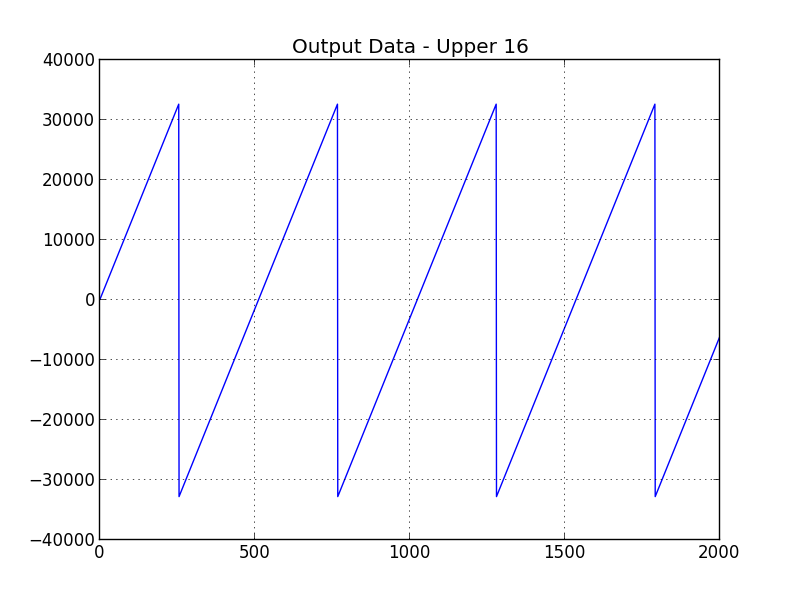
\includegraphics[scale=0.5]{./figures/upper16.jpg}
                \caption{``RAMP'' Output (Passed through by ``ANDER'')}
                \label{fig:upper16}
        \end{figure}

        \begin{figure}[H]
                \centering
                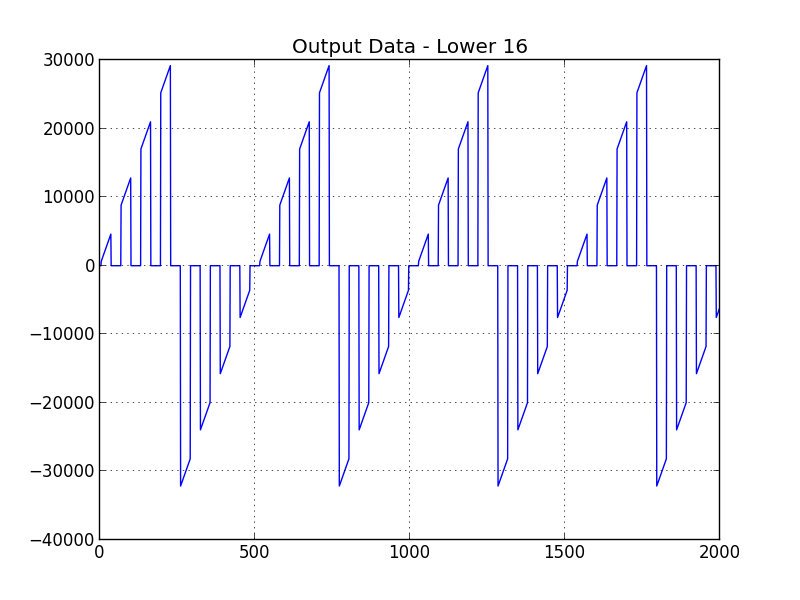
\includegraphics[scale=0.5]{./figures/lower16.jpg}
                \caption{``ANDER'' Output}
                \label{fig:lower16}
        \end{figure}
\bend
\bstart
For completeness, the output plot of the \verb+square+ \textit{component} is provided in Figure \ref{fig:square_pulse}. The steps to generate a unit test for the \verb+square+ \textit{component} are outside the scope of this document.

        \begin{figure}[H]
                \centering
                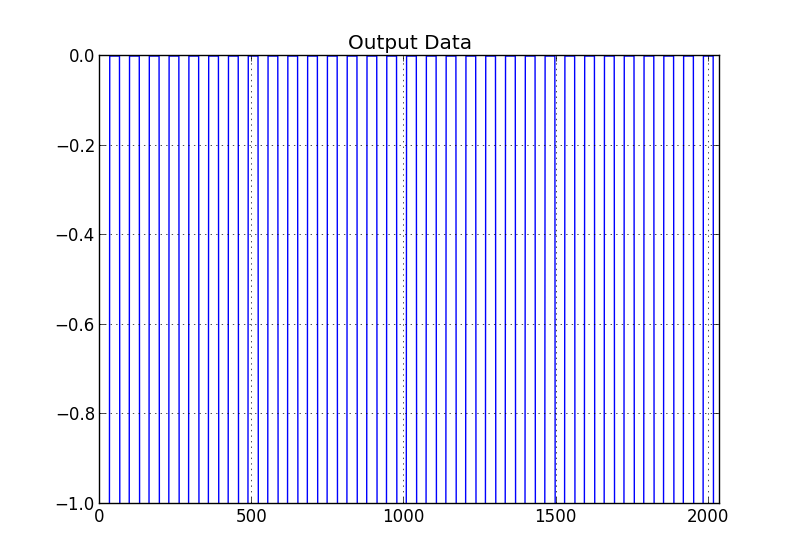
\includegraphics[scale=0.5]{./figures/square_pulse.jpg}
                \caption{``SQUARE'' Output = Input 2 to ``ANDER''}
                \label{fig:square_pulse}
        \end{figure}
\bend
\bstart
\subsection{Adding Backpressure}
For more realistic testing, the ``\path{backpressure}'' component can simulate downstream components being ``too busy'' to receive data. By default, all unit tests of a \textit{single} component includes backpressure to assist development (see the \textit{Component Development Guide}). This section adds the \path{backpressure} component between the \path{ander} and \path{file_write}. If \path{ander} properly implements backpressure, it will indicate to \path{ramp} and \path{square} that they should not push more data to it. If they properly handle backpressure, they will halt their generation routines and avoid a discontinuity in their output.
\subsubsection*{New Assembly XML}
Replace the existing assembly XML (from~\sref{example:assembly}) with the following code:
\begin{lstlisting}[language=xml]
<HdlAssembly>
<Instance Worker="file_read" Connect="ramp"/>
  <Instance Worker="ramp" />
  <Instance Worker="square"/>
  <Instance Worker="ander" Connect="backpressure"/>
  <Instance Worker="backpressure" Connect="file_write"/>
  <Instance Worker="file_write"/>
  <Connection>
    <Port Instance="ramp" Name="out"/>
    <Port Instance="ander" Name="in1"/>
  </Connection>
  <Connection>
    <Port Instance="square" Name="out"/>
    <Port Instance="ander" Name="in2"/>
  </Connection>
</HdlAssembly>
\end{lstlisting}
\bend
\bstart
\subsubsection*{New Application XML}
Replace the existing application XML (from~\sref{example:application}) with the following code:
\begin{lstlisting}[language=xml]
<Application>
  <Instance Component="ocpi.core.file_read" Connect="ramp">
    <Property Name="fileName" Value="idata/input_file.bin"/>
  </Instance>
  <Instance Component="local.DemoProject.ramp"/>
  <Instance Component="local.DemoProject.square"/>
  <Instance Component="local.DemoProject.ander" Connect="backpressure"/>
  <Instance Component="ocpi.core.backpressure" Connect="file_write">
    <property name='enable_select' value='true'/>
  </Instance>
  <Instance Component="ocpi.core.file_write">
    <Property Name="fileName" Value="odata/output_file.bin"/>
  </Instance>
  <Connection>
    <Port Instance="ramp" Name="out"/>
    <Port Instance="ander" Name="in1"/>
  </Connection>
  <Connection>
    <Port Instance="square" Name="out"/>
    <Port Instance="ander" Name="in2"/>
  </Connection>
</Application>
\end{lstlisting}
\bend
\bstart
\subsubsection*{Results}
Once the workers (\sref{example:buildworkers}) and assemblies (\sref{example:buildasms}) are rebuilt, the application's results (Sections~\ref{example:run}~and~\ref{example:output}) should be exactly as the output \textit{without} backpressure. If not, the HDL workers will most likely drop data when deployed to a non-simulation platform.
\bend

%\todo{recap what was learned as a closing}

\section{Other Example Applications}
For more examples, please consult:
\begin{itemize}
  \item \githubio[\textit{FSK App RCC Getting Started Guide}]{assets/FSK\_App\_RCC\_Getting\_Started\_Guide.pdf} for a software-only variant of the FSK App (described below)
  -- \textbf{this is the only demonstration that will execute end-to-end on a CentOS system without additional software installed, \textit{e.g.} a simulator}.
  \item \githubio[\textit{FSK App Getting Started Guide}]{assets/FSK\_App\_Getting\_Started\_Guide.pdf} for an FPGA-based FSK Example, including RF TX and RX.
  \item More detailed examples and presentation slides available as ``Standalone Training'' on \href{http://opencpi.github.io/}{\path{github.io}}.
\end{itemize}

\end{document}
